\documentclass[11pt]{article}
\usepackage[margin=1in]{geometry}
\usepackage{amsmath,amssymb,mathtools}
\usepackage{tikz}
\usetikzlibrary{arrows.meta,positioning}
\title{TaxonomyGraphVAE: Mathematical Formulation}
\date{}
\begin{document}
\maketitle

\section{Graph encoder}
With weighted adjacency $A$, define
\begin{equation}
\tilde A=A+I,\qquad \hat A=D^{-1/2}\tilde A D^{-1/2},\qquad D_{ii}=\sum_j\tilde A_{ij}.
\end{equation}
Starting from $H^{(0)}=I_n$, propagation layers are
\begin{equation}
H^{(\ell+1)}=\sigma\!\left(\hat A H^{(\ell)}W^{(\ell)}+b^{(\ell)}\right).
\end{equation}
Feature embeddings (for taxonomy-linked feature nodes $S$) are
\begin{equation}
E=H^{(L)}_{S,:}\in\mathbb R^{p\times d_g}.
\end{equation}

\section{Sample pooling}
For sample $x\in\mathbb R^p$, construct nonnegative normalized weights $w$ (uniform fallback if degenerate), then
\begin{equation}
r(x)=w^\top E\in\mathbb R^{d_g}.
\end{equation}

\section{VAE parameterization}
\begin{equation}
(\mu,\log\sigma^2)=g_\phi(r(x)),
\quad
q_\phi(z\mid x)=\mathcal N(\mu,\operatorname{diag}(\sigma^2)),
\quad
p(z)=\mathcal N(0,I).
\end{equation}
\begin{equation}
z=\mu+\sigma\odot\varepsilon,\; \varepsilon\sim\mathcal N(0,I),
\qquad
\hat x=f_\theta(z).
\end{equation}

\section{Objective}
\begin{equation}
\mathcal J(x)=\mathcal L_{\mathrm{rec}}(x,\hat x)+\beta_t\,\mathrm{KL}(q_\phi(z\mid x)\|p(z)).
\end{equation}

\section{Diagram}
\begin{center}
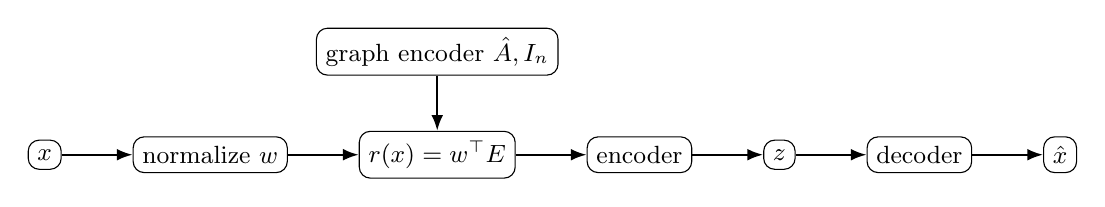
\begin{tikzpicture}[node distance=7mm and 9mm, box/.style={draw,rounded corners,align=center,font=\small}, arr/.style={-{Latex[length=2mm]},thick}]
\node[box] (x) {$x$};
\node[box,right=of x] (w) {normalize $w$};
\node[box,right=of w] (pool) {$r(x)=w^\top E$};
\node[box,above=of pool] (gnn) {graph encoder $\hat A,I_n$};
\node[box,right=of pool] (enc) {encoder};
\node[box,right=of enc] (z) {$z$};
\node[box,right=of z] (dec) {decoder};
\node[box,right=of dec] (xh) {$\hat x$};
\draw[arr] (x)--(w); \draw[arr] (w)--(pool); \draw[arr] (gnn)--(pool); \draw[arr] (pool)--(enc); \draw[arr] (enc)--(z); \draw[arr] (z)--(dec); \draw[arr] (dec)--(xh);
\end{tikzpicture}
\end{center}
\end{document}
